\documentclass[10pt,twocolumn]{article}

\usepackage[a4paper, top=30mm, bottom=20mm, left=10mm, right=10mm]{geometry}
\usepackage[hangul]{kotex}
\newcommand{\titleko}{자연 연역 체계의 전산화에 관한 연구}
\newcommand{\titleen}{On computerizing natural deduction}
\newcommand{\authorname}{이상길}
\newcommand{\getkeywords}{수학기초론, 형식주의, 람다 계산법, 자연 연역 체계}
\usepackage[pdfencoding=unicode,
	pdfauthor={\authorname},
	pdftitle={\titleko},
	pdfkeywords={\getkeywords},
	bookmarks]{hyperref}
\usepackage{amsmath, amscd, amsthm, amssymb, amsfonts, mathrsfs, mathtools, mathalfa}
\usepackage{abstract}
\usepackage[sans]{dsfont}
\usepackage{latexsym}
\usepackage{enumitem}
\usepackage{color}
\usepackage{url}
\usepackage{graphicx}
\graphicspath{{./images/}}
\usepackage{multirow}
\usepackage{float}
\usepackage{listings}
\usepackage[square,numbers]{natbib}
\bibliographystyle{ieeetr}
\usepackage{caption}
% \captionsetup[table]{skip=.5em}
\usepackage{fitch}
\usepackage{bm}
\usepackage{adjustbox}

\definecolor{javared}{rgb}{0.6,0,0}
\definecolor{javapurple}{rgb}{0.5,0,0.35}

\lstdefinelanguage{mom}{
	keywords={type,axiom,theorem},
	sensitive=true,
	keywordstyle=\color{javapurple}\ttfamily,
	morecomment=[s][\color{javared}]{<}{>},
}

\lstset{
	language=mom,
	basicstyle=\small\ttfamily,
	numberstyle=\small\ttfamily,
	tabsize=4,
	numbers=left,
	xleftmargin=.7cm
}

\theoremstyle{definition}
\newtheorem{theorem}{정리}
\newtheorem{definition}[theorem]{정의}
\newtheorem{example}[theorem]{예시}

\newcommand{\N}{\mathbb{N}}
\newcommand{\Z}{\mathbb{Z}}
\newcommand{\Q}{\mathbb{Q}}
\newcommand{\R}{\mathbb{R}}

\newcommand{\sinc}{\operatorname{sinc}}
\newcommand{\dom}{\operatorname{dom}}
\newcommand{\im}{\operatorname{im}}
\newcommand{\ord}{\operatorname{ord}}
\newcommand{\Prop}{\mathsf{Prop}}
\newcommand{\Cls}{\mathsf{Cls}}
\newcommand{\Predicate}{\mathsf{Predicate}}
\newcommand{\leqnormal}{\mathrel{\unlhd}}
\newcommand{\ltnormal}{\mathrel{\lhd}}

\newcommand{\lch}{\bm\lambda_\to^{\text{Ch}}}
\newcommand{\lchh}{\bm\lambda_{\to,\vdash}^{\text{Ch}}}
\newcommand{\Lch}{\Lambda_\to^{\text{Ch}}}
\newcommand{\Lchh}{\Lambda_{\to,\vdash}^{\text{Ch}}}

\newcommand{\fv}{\mathbf{FV}}
\newcommand{\bv}{\mathbf{BV}}

% \renewcommand{\abstractname}{초 록}
\renewcommand{\refname}{참고문헌}
\kscntformat{section}{}{}

\title{\titleko%\\[1ex]\large\titleen
}
\author{\authorname\thanks{\href{mailto:ossia@korea.ac.kr}{\texttt{ossia@korea.ac.kr}}}}
\date{}

\begin{document}

\twocolumn[
\begin{@twocolumnfalse}
	\maketitle
	\begin{abstract}
		\centering\begin{minipage}{\dimexpr\paperwidth-8cm}
			\noindent 우리는 엄밀하면서도 읽고 쓰기 쉬운 증명을 작성할 수 있도록 자연 연역 체계를 전산화하였으며, 이를 위해 단순 타입 람다 계산법에 기반하여 형식 언어를 구축하였다. 우리의 자연 연역 체계는 증명 체계의 동작 방식을 묘사할 수 있는 능력을 가지며, 이는 사용자가 형식 언어 및 공리, 추론 규칙을 자유롭게 정할 수 있도록 한다. 우리는 증명 체계를 만들고, 만들어진 증명 체계에서 컴퓨터에 의해 검증되는 증명을 할 수 있도록 하는 웹 기반 컴퓨터 프로그램 \texttt{math-o-matic}을 만들었으며, Morse--Kelly 집합론을 기반으로 하여 이항관계 및 함수, 자연수 집합, 정수 집합에 관한 개념을 정의하고 관련 정리를 증명할 수 있었다.
			
			\smallskip\noindent {\bf 주제어}: \getkeywords
		\end{minipage}
	\end{abstract}\vspace{2em}\vspace{1.5em}
\end{@twocolumnfalse}
]

\saythanks

\section{서론}

수학적 형식주의의 관점에서 모든 수학적 정의 및 정리는 어떤 증명 체계(proof system) 상에서 표현할 수 있으며, 곧 증명 체계는 수학 전체를 표현할 수 있는 능력을 갖는다. 이때 증명 체계 상에서 이루어지는 증명은 그 형식적 특성에 의하여 컴퓨터에 의해 기계적으로 검증될 수 있으며, 이는 증명 과정에서 발생할 수 있는 실수를 배제한다. 그러므로 증명 체계를 전산화하는 것이 필요하며, 우리는 엄밀하면서도 읽고 쓰기 쉬운 증명을 작성할 수 있도록 가언적 추론(假言的推論, hypothetical derivation)을 지원하는 자연 연역 체계를 전산화하기로 하였다.

증명 체계를 만들기 위해서는 먼저 증명 체계가 사용할 형식 언어를 만들어야 한다. 이때 잘못된 문장을 구성하는 것을 방지하기 위하여 언어 상의 모든 용어는 타입을 갖도록 할 것인데, 예를 들어 ``$1+1=2$''라는 명제는 명제 타입 $\Prop$을 가질 것이고, 연언(連言)을 뜻하는 이항연산자 $\land$는 두 개의 명제를 받아 새로운 명제를 만드는 함수이므로 $\Prop\times\Prop\to\Prop$ 타입을 가질 것이다. 이때 $p$ 및 $q$가 명제인 경우 $p\land q$는 이항연산자 $\land$에 인자 $(p, q)$를 주어 호출한 것이며 $p\land q$의 타입은 $\land$의 반환 타입인 $\Prop$이 된다. 예시로부터 알 수 있듯 우리의 언어는 함수의 생성 및 호출에 관한 구문을 지원하여야 하며, 곧 특정 조건을 만족하는 람다 항의 집합이 되어야 한다. 우리는 단순 타입 람다 계산법(simply typed lambda calculus)에 기반하여 언어를 구축할 것이다.

또 우리의 체계는 형식 언어 및 공리, 추론 규칙을 미리 정해 두지 않고 우리의 체계를 활용하려는 자가 임의로 정할 수 있도록 하려고 하며, 이를 위하여 우리의 언어는 추론 규칙에 대한 표현력을 가진다. 예를 들어 Hilbert 체계의 대표적 추론 규칙인 함의 소거(implication elimination) $p, p\to q\vdash q$는 $\vdash$를 포함하는 메타문장이므로 대상언어에 속하지 않으나, 우리의 체계는 이를 언어에 포함시킨다. 그러므로 우리의 언어를 구성하기 위해서는 단순 타입 람다 계산법에 $\vdash$ 구문을 추가할 필요가 있다. 이때 우리의 증명 체계는 $\vdash$ 구문이 추론 규칙처럼 작동할 수 있도록 하는 추론 규칙들을 가진다.

문제는 $\vdash$ 구문을 추가하여도 함의 소거가 메타변항(metavariable) $p$ 및 $q$를 포함하는 스키마(schema)이므로 대상언어에 속할 수 없다는 것이다. 이를 해결하기 위하여 우리는 스키마를 메타변항들을 매개변항으로 하는 함수라고 생각하여 메타변항들을 종속시킬 것이다. 예를 들어 함의 소거는 명제 $p$ 및 $q$를 받아 $p, p\to q\vdash q$를 반환하는 함수가 된다. 이때 우리의 증명 체계는 함수로 표현한 스키마들이 스키마처럼 작동할 수 있도록 하는 추론 규칙들을 가질 것이다.

즉 우리의 체계는 증명 체계의 동작 방식을 묘사하는 증명 체계이다. 또 우리의 체계는 람다 계산법을 활용한 자연 연역 체계임에도 불구하고 람다 계산법의 타입 체계와 자연 연역 체계 간의 Curry--Howard 대응\cite{howard}에 의존하지 않는다. 이는 수식을 타입이 아니라 람다 항이라 생각하기 때문이며, 이로 인해 어떤 정리의 증명 가능성과 type inhabitation 문제가 대응된다는 해석을 받아들이지 않아도 된다는 점에서 더 직관적이다.

\section{형식 언어의 정의}

$\lch$가 \cite{luswt}의 정의~1.1.30과 같이 정의된다고 하자. $\lch$에서는 모든 변항(變項)에 고유한 타입이 지정되어 있어서 타이핑 문맥(typing context)이 필요하지 않다. 이제 $\lch$에 $\vdash$ 구문을 추가하여 새로운 체계 $\lchh$를 만들어 보자. 먼저 타입 생성자 $\vdash$를 추가하기 위하여 \cite{luswt}의 정의~1.1.11의 BNF를 다음과 같이 수정하자.
$$\mathds T \Coloneqq \mathbb A\mid\mathds T\to\mathds T\mid\mathds T\vdash\mathds T.$$
또 $M\vdash N$ 형태의 람다 항이 생성될 수 있도록 \cite{luswt}의 정의~1.1.30(ii)에 다음과 같은 규칙을 추가하자.
$$M\in\Lchh(A), N\in\Lchh(B)\Rightarrow (M\vdash N)\in\Lchh(A\vdash B).$$
$\vdash$는 오른쪽 결합성을 갖는다고 하자. 즉 $p\vdash q\vdash r$는 $p\vdash (q\vdash r)$를 뜻한다. $\vdash$ 구문이 전건을 하나만 가질 수 있도록 하는 것은 추상화 구문에서 매개변항을 하나만 지정할 수 있는 것과 같은 이유로, $\vdash$ 구문에 커링(currying)을 적용하여
$$p_1, p_2, \ldots, p_n\vdash q$$
를
$$p_1 \vdash p_2\vdash\cdots\vdash p_n\vdash q$$
로 표현할 수 있기 때문이다.

또 우리 체계는 함수의 외연성(extensionality)을 받아들여 $\bm{\lambda\beta\eta}$를 equational theory로 사용할 것인데, $\vdash$에 대한 합동을 고려하기 위하여 규칙
$$\dfrac{M=M'\quad N=N'}{(M\vdash N)=(M'\vdash N')}$$
을 추가하여야 한다. 이때 Church식 의미론에 의하여 $A\ne B$일 때 $\lambda x^A.x^A\ne\lambda x^B.x^B$이다. 이제 $\beta\eta$ 동치인 두 람다 항은 서로 같다고 볼 것이다.

또 $\land$나 $\forall$ 등의 무정의용어를 도입하기 위해서는 정항(正項)을 추가할 수 있어야 하는데, 정항의 집합 $\mathcal C$는 \cite{luswt}의 정의~1.1.30(i)에서 정의된 변항의 집합 $\mathsf V^{\mathds T}$의 부분집합으로 정의하자. 이때 우리의 형식 언어 $\mathcal L$은 다음과 같이 정의된다.

\begin{definition}[형식 언어]
	$\mathbb A$가 원시 타입의 집합이고 $\mathds T = \mathds T^{\mathbb A}$일 때, 정항의 집합 $\mathcal C\subseteq \mathsf V^{\mathds T}$에 대하여 형식 언어 $\mathcal L$이 다음과 같이 정의된다.
	$$\mathcal L = \{M\in\Lchh: \mathrm{FV}(M)\subseteq\mathcal C\}.$$
\end{definition}

즉 $\mathcal L$은 $\Lchh$에 있는 람다 항 중에서 자유 변항이 전부 정항인 것들의 집합이다.

\section{공리 및 추론 규칙의 정의}

가정의 집합 $\Gamma\subseteq\Lchh$ 및 람다 항 $\varphi\in\Lchh$에 대해 시퀀트(sequent)가 $\Gamma\Rightarrow\varphi$ 형태의 식을 뜻한다고 하자. $\Gamma\Rightarrow\varphi$는 ``가정 $\Gamma$로부터 $\varphi$를 증명할 수 있다"는 뜻이라 생각할 수 있다. 우리의 증명 체계는 증명 체계의 동작을 모사하는 5개의 추론 규칙을 가진다.

\begin{definition}[공리 및 추론 규칙]
	우리 증명 체계의 공리 및 추론 규칙은 다음과 같다.
	
	\begin{enumerate}
		\item (R 규칙)\quad 임의의 $\varphi\in\Gamma$에 대하여 $\Gamma\Rightarrow\varphi.$
		\item ($\vdash$E 규칙)\quad $\dfrac{\Gamma\Rightarrow\varphi\quad\Gamma\Rightarrow(\varphi\vdash\psi)}{\Gamma\Rightarrow\psi}.$
		\item ($\vdash$I 규칙)\quad $\dfrac{\Gamma\cup\{\varphi\}\Rightarrow\psi}{\Gamma\Rightarrow(\varphi\vdash\psi)}.$
		\item ($\mapsto$E 규칙)\quad $\varphi\psi\in\Lchh$일 때 $$\dfrac{\Gamma\Rightarrow\varphi}{\Gamma\Rightarrow\varphi\psi}.$$
		\item ($\mapsto$I 규칙)\quad $x^A\notin\mathcal C$일 때 $$\dfrac{\Gamma\Rightarrow\varphi}{\Gamma\Rightarrow\lambda x^A.\varphi}.$$
	\end{enumerate}
\end{definition}

공리 및 추론 규칙이 모두 시퀀트에 관한 것인 이유는 우리 체계가 가언적 추론을 지원하는 자연 연역 체계이기 때문이다. 이때 $\vdash$E 및 $\vdash$I 규칙에 의하여 $\vdash$ 구문이 추론 규칙처럼 작동하며 $\mapsto$E 및 $\mapsto$I 규칙에 의하여 함수로 표현한 스키마들이 스키마처럼 작동한다. 특히 $\vdash$I 규칙은 유도 가능한 규칙(derivable rule)을 유도할 수 있도록 하며, 이로 인하여 우리 체계가 가언적 추론을 지원하게 된다.

\begin{example} \label{example:proof}
	$$\Gamma = \left\{\begin{array}{l}
		\lambda p^\Prop\lambda q^\Prop.(p\vdash(q\vdash {\land}pq)),\\
		\lambda p^\Prop\lambda q^\Prop.({\land}pq\vdash p),\\
		\lambda p^\Prop\lambda q^\Prop.({\land}pq\vdash q)
	\end{array}\right\}$$
	일 때
	$$\Gamma\Rightarrow\lambda p^\Prop\lambda q^\Prop.({\land}pq\vdash{\land}qp)$$
	는 그림~\ref{fig:proof1}\과 같이 증명할 수 있으며, 이는 Fitch 다이어그램으로 그림~\ref{fig:proof2}\와 같이 더 간단히 표현할 수 있다. 단 그림~\ref{fig:proof2}에서 연속된 $\mapsto$E 또는 $\vdash$E, $\mapsto$I는 하나로 표현되었다.
	
	\begin{figure}[bt] \centering\small\fbox{
		\begin{tabular}{lll}
			1 & $\Gamma\cup\{{\land}p'q'\}\Rightarrow {\land}p'q'$ & R \\
			2 & $\Gamma\cup\{{\land}p'q'\}\Rightarrow \lambda p\lambda q.({\land}pq\vdash p)$ & R \\
			3 & $\Gamma\cup\{{\land}p'q'\}\Rightarrow \lambda q.({\land}p'q\vdash p')$ & $\mapsto$E (2) \\
			4 & $\Gamma\cup\{{\land}p'q'\}\Rightarrow ({\land}p'q'\vdash p')$ & $\mapsto$E (3) \\
			5 & $\Gamma\cup\{{\land}p'q'\}\Rightarrow p'$ & $\vdash$E (1, 4) \\
			6 & $\Gamma\cup\{{\land}p'q'\}\Rightarrow \lambda p\lambda q.({\land}pq\vdash q)$ & R \\
			7 & $\Gamma\cup\{{\land}p'q'\}\Rightarrow \lambda q.({\land}p'q\vdash q)$ & $\mapsto$E (6) \\
			8 & $\Gamma\cup\{{\land}p'q'\}\Rightarrow ({\land}p'q'\vdash q')$ & $\mapsto$E (7) \\
			9 & $\Gamma\cup\{{\land}p'q'\}\Rightarrow q'$ & $\vdash$E (1, 8) \\
			10 & $\Gamma\cup\{{\land}p'q'\}\Rightarrow \lambda p\lambda q.(p\vdash (q\vdash{\land}pq))$ & R \\
			11 & $\Gamma\cup\{{\land}p'q'\}\Rightarrow \lambda q.(q'\vdash(q\vdash{\land}q'q))$ & $\mapsto$E (10) \\
			12 & $\Gamma\cup\{{\land}p'q'\}\Rightarrow (q'\vdash(p'\vdash{\land}q'p'))$ & $\mapsto$E (11) \\
			13 & $\Gamma\cup\{{\land}p'q'\}\Rightarrow (p'\vdash{\land}q'p')$ & $\vdash$E (9, 12) \\
			14 & $\Gamma\cup\{{\land}p'q'\}\Rightarrow {\land}q'p'$ & $\vdash$E (5, 13) \\
			15 & $\Gamma\Rightarrow ({\land}p'q'\vdash {\land}q'p')$ & $\vdash$I (14) \\
			16 & $\Gamma\Rightarrow \lambda q'.({\land}p'q'\vdash {\land}q'p')$ & $\mapsto$I (15) \\
			17 & $\Gamma\Rightarrow \lambda p'\lambda q'.({\land}p'q'\vdash {\land}q'p')$ & $\mapsto$I (16) \\
			& \qquad\quad$=\lambda p\lambda q.({\land}pq\vdash {\land}qp)$ & $\alpha$ 동치
		\end{tabular}}
		\caption{$\Gamma\Rightarrow \lambda p^\Prop\lambda q^\Prop.({\land}pq\vdash{\land}qp)$의 증명} \label{fig:proof1}
	\end{figure}
	
	\begin{figure}[bt] \centering\small\fbox{
		$\begin{nd}\close
			\open[p']
			\open[q']
			\open
			\hypo{}{{\land}p'q'} \by{가정}{}
			\have{}{\lambda p\lambda q.({\land}pq\vdash p)} \by{R}{}
			\have{}{{\land}p'q'\vdash p'} \by{$\mapsto$E (2)}{}
			\have{}{p'} \by{$\vdash$E (1, 3)}{}
			\have{}{\lambda p\lambda q.({\land}pq\vdash q)} \by{R}{}
			\have{}{{\land}p'q'\vdash q'} \by{$\mapsto$E (5)}{}
			\have{}{q'} \by{$\vdash$E (1, 6)}{}
			\have{}{\lambda p\lambda q.(p\vdash (q\vdash{\land}pq))} \by{R}{}
			\have{}{q'\vdash(p'\vdash{\land}q'p')} \by{$\mapsto$E (8)}{}
			\have{}{{\land}q'p'} \by{$\vdash$E (7, 4, 9)}{}
			\close
			\have{}{{\land}p'q'\vdash {\land}q'p'} \by{$\vdash$I (1--10)}{}
			\close
			\close
			\have{}{\lambda p\lambda q.({\land}pq\vdash {\land}qp)} \by{$\mapsto$I (1--11)}{}
		\end{nd}$}
		\caption{Fitch 다이어그램으로 표현한 증명} \label{fig:proof2}
	\end{figure}
\end{example}

\section{증명 체계의 정의}

증명 체계는 원시 타입의 집합 $\mathbb A$, 정항의 집합 $\mathcal C\subseteq\mathsf V^{\mathds T}$, 공리의 집합 $\Gamma_0\subseteq\mathcal L$에 의해 결정된다. 이때 어떤 명제 $\varphi\in\mathcal L$이 체계 $\langle\mathbb A,\mathcal C,\Gamma_0\rangle$ 상에서 증명 가능하다는 것은 다음과 같은 뜻이다.

\begin{definition}[증명 가능성]
	$\langle\mathbb A,\mathcal C,\Gamma_0\rangle$ 상에서 $\varphi\in\mathcal L$이 증명 가능하다는 것은 $\Gamma_0\Rightarrow\varphi$가 유도 가능하다는 뜻이다.
\end{definition}

이제부터 함수 타입 및 $\vdash$ 타입을 언커링(uncurrying) 하여 표시하자. $\lambda x^A\ldots\lambda z^C.M$은 $(x^A, \ldots, z^C)\mapsto M$이라 쓰자. 또 $fxy$ 대신 $f(x, y)$라 쓰고 $p\vdash q\vdash r$ 대신 $p, q\vdash r$라 쓰자. $\land$ 등의 이항연산자의 경우 ${\land}(p, q)$ 대신 $p\land q$라고도 쓸 수 있다.

\begin{example}\label{example:system}
	명제논리를 위한 증명 체계는 다음과 같이 정의해 볼 수 있다.
	\begin{align*}
		\mathbb A &= \{\mathsf{Prop}\}, \\
		\mathcal C &= \{\to, \neg, \land, \top\}, \\
		\Gamma_0 &= \left\{\begin{array}{l}
			(p^\Prop, q^\Prop)\mapsto \left((p\vdash q)\vdash p\to q\right), \\
			(p^\Prop, q^\Prop)\mapsto \left(p, p\to q\vdash q\right), \\
			(p^\Prop, q^\Prop)\mapsto \left(p, q\vdash p\land q\right), \\
			(p^\Prop, q^\Prop)\mapsto \left(p\land q\vdash p\right), \\
			(p^\Prop, q^\Prop)\mapsto \left(p\land q\vdash q\right), \\
			\top, \\
			(p^\Prop, q^\Prop)\mapsto \left(\neg p\to\neg q\vdash q\to p\right)
		\end{array}\right\}.
	\end{align*}
\end{example}

\subsection{매크로의 정의}

예시~\ref{example:system}의 체계에는 $\lor$, $\leftrightarrow$ 연산자 및 $\bot$도 정의되어 있는데 이들은 무정의용어로서가 아닌 다른 개념에 의존하는 매크로로서 정의되어 있으므로 무정의용어의 집합인 $\mathcal C$에 나타나지 않는다. 이들은 다음과 같이 정의되어 있다.
\begin{align*}
	\lor&\coloneqq (p^\Prop, q^\Prop)\mapsto \left(\neg p\to q\right), \\
	\leftrightarrow&\coloneqq (p^\Prop, q^\Prop)\mapsto \left((p\to q)\land(q\to p)\right), \\
	\bot&\coloneqq\neg\top.
\end{align*}
또 Morse--Kelley 집합론에서 단항 술어는 클래스 하나를 받아 명제를 출력하는 함수이므로 $\Cls\to\Prop$ 타입일 것이며, 이 역시 매크로로서
$$\Predicate\coloneqq\Cls\to\Prop$$
이라 정의할 수 있다.

\section{\texttt{math-o-matic}: 전산화된 증명 체계}

우리는 증명 체계 $\langle\mathbb A, \mathcal C, \Gamma_0\rangle$을 만들고, 만들어진 증명 체계에서 컴퓨터에 의해 검증되는 증명을 할 수 있도록 하는 웹 기반 컴퓨터 프로그램을 만들었으며 이름을 \texttt{math-o-matic}이라 하였다. \texttt{math-o-matic}의 소스 코드 및 \texttt{math-o-matic}을 실행할 수 있는 웹 페이지는
\begin{center}\small
	\href{https://github.com/logico-philosophical/math-o-matic}{\texttt{https://github.com/logico-philosophical/math-o-matic}}
\end{center}
에서 찾을 수 있다.

\texttt{math-o-matic}은 증명 체계의 정의 및 증명 작성을 위한 기술 언어를 제공한다. 예를 들어 타입 $\Prop$ 및 무정의용어 $\land$를 정의하고, 예시~\ref{example:proof}의 $\Gamma$를 공리계에 포함시키는 코드는 다음과 같이 작성할 수 있다.

\begin{lstlisting}
type Prop;

Prop A(Prop p, Prop q);

axiom Ai(Prop p, Prop q) {
	p, q |- A(p, q)	
}

axiom Ae1(Prop p, Prop q) {
	A(p, q) |- p
}

axiom Ae2(Prop p, Prop q) {
	A(p, q) |- q	
}
\end{lstlisting}
단 \verb!A!가 $\land$를 뜻한다. 이때 그림~\ref{fig:proof2}의 증명은 다음과 같이 작성할 수 있다.
\begin{lstlisting}
theorem A_flip(Prop p, Prop q) {
	A(p, q) |- {
		[
			@h1 > Ae2(p, q);
			@h1 > Ae1(p, q)
		] > Ai(q, p)
	}
}
\end{lstlisting}
둘째 줄이 가정 \verb!A(p, q)!를 도입하며 \verb!@h1!이 이를 가리킨다. \verb!Ae2(p, q)!는 \verb!Ae2!를 인자 \verb!(p, q)!로 호출하므로 넷째 줄은
\begin{center}
	\verb!A(p, q) > (A(p, q) |- q)!
\end{center}
가 되며, \verb!>! 연산자는 좌변 \verb!A(p, q)!와 우변의 전건 \verb!A(p, q)!를 비교하여 이들이 $\beta\eta$ 동치이면 우변의 후건 \verb!q!를 유도한다. 그러므로 넷째 줄이 \verb!q!가 되고 같은 방식으로 다섯째 줄이 \verb!p!가 되므로, 3--6번째 줄은
\begin{center}
	\verb![q; p] > (q, p |- A(q, p))!
\end{center}
가 되며 이것이 \verb!A(q, p)!를 유도한다. 그러므로 2--7번째 줄이
\begin{center}
	\verb!A(p, q) |- A(q, p)!
\end{center}
가 되어 $(p^\Prop, q^\Prop)\mapsto (p\land q\vdash q\land p)$가 증명된다.

\texttt{math-o-matic} 프로그램은 위의 증명을 검증하고 그림~\ref{fig:Aflip}\과 같이 Fitch 다이어그램으로 표시할 수 있다. 이때 표현의 간결함을 위하여 R, $\vdash$I, $\mapsto$E, $\mapsto$I 규칙의 적용은 생략되었으며, 추가적인 코드를 작성하여 \verb!A(p, q)!가 $p\land q$로 표시되도록 하였다.

\begin{figure}[bt!] \centering
	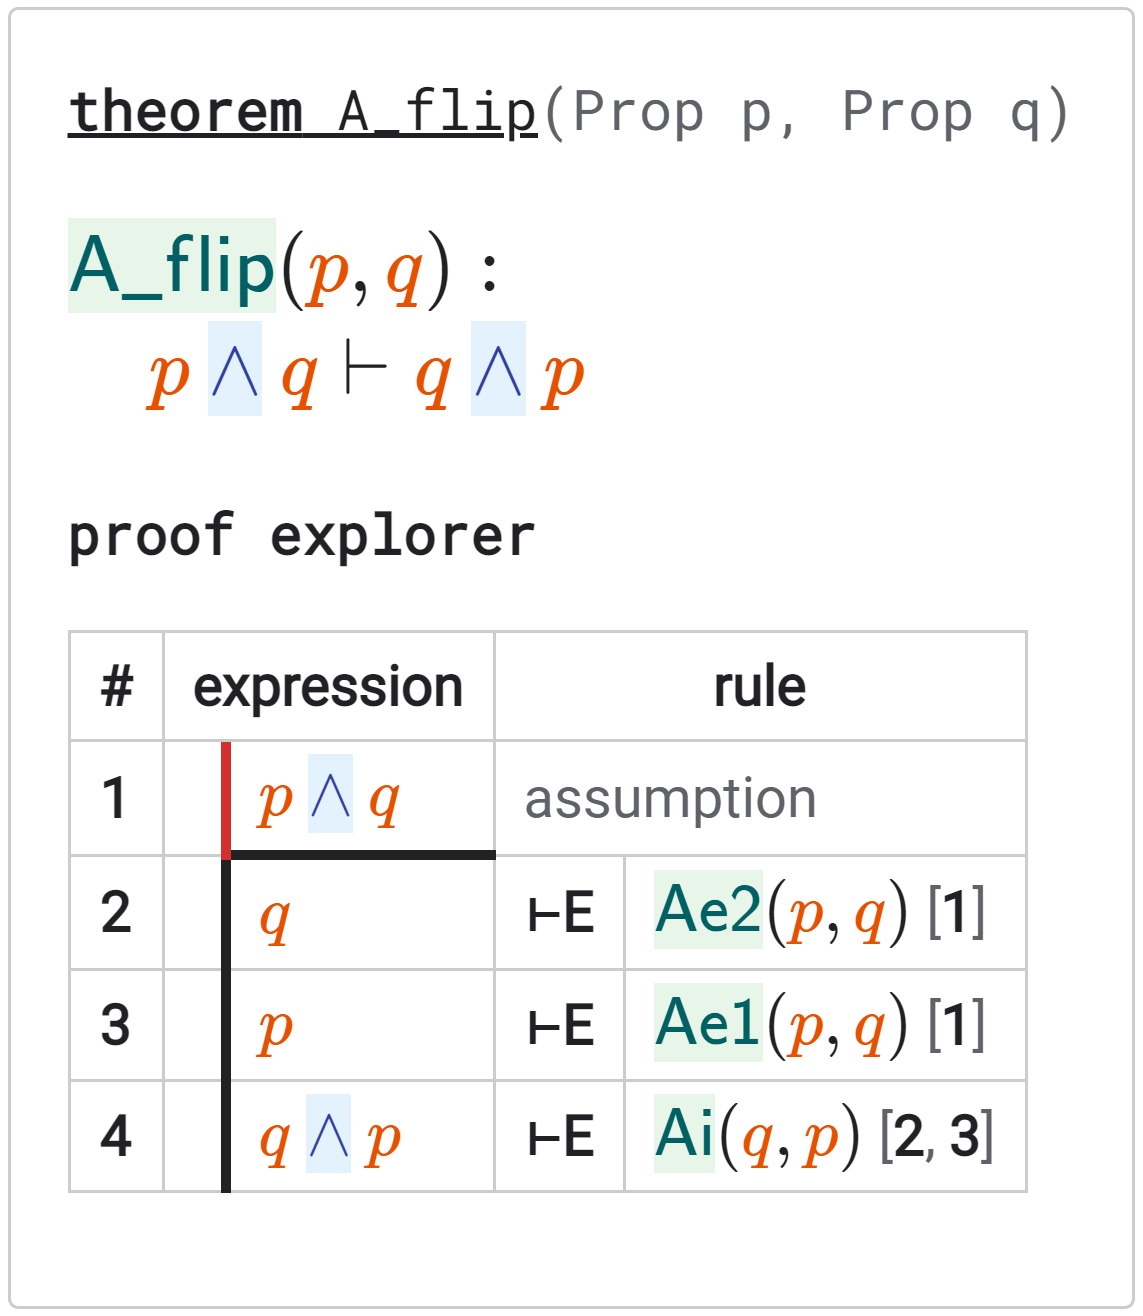
\includegraphics[scale=.18]{A_flip}
	\caption{\texttt{A\_flip}의 증명} \label{fig:Aflip}
\end{figure}


\section{수학의 전산화}

우리는 \texttt{math-o-matic} 체계 상에서 Morse--Kelley 집합론을 기반으로 하여 이항관계 및 함수, 자연수 집합, 정수 집합에 관한 개념을 정의하고 관련 정리들을 증명할 수 있었으며, 이들은 \texttt{math-o-matic} 메인 페이지에서 확인할 수 있다. 현재 $\langle\mathbb A, \mathcal C, \Gamma_0\rangle$은 다음과 같이 정의되어 있다.

\begin{description}[leftmargin=0cm]
	\item[원시 타입.] $\Prop$ 및 $\Cls$ 두 개가 있다.
	\item[무정의용어.] 8개의 무정의용어가 있으며, 명제논리를 위한 무정의용어는 예시~\ref{example:system}에서와 같이 $\to$, $\neg$, $\land$, $\top$이다. 술어논리를 위한 무정의용어는 $\forall$ 하나이며, 타입 $\Predicate\to\Prop$을 갖는다. 이는 $(\forall x)(f(x))$를 $\forall(x\mapsto f(x))$라고 생각한 것이다. 집합론을 위한 무정의용어는 $=$, $\in$ 및 조건제시법(set-builder notation)이 있다.
	\item[공리계.] 17개의 공리가 정의되어 있으며, 명제논리를 위한 공리계는 예시~\ref{example:system}의 $\Gamma_0$와 같다. 또 술어논리를 위한 공리는 다음의 두 개 뿐이다.
	\begin{align*}
		(f^\Predicate)&\mapsto (f\vdash\forall f), \\
		(f^\Predicate, x^\Cls)&\mapsto (\forall f\vdash f(x)).
	\end{align*}
	이외의 공리는 모두 Morse--Kelley 집합론의 공리를 가져온 것이다.
\end{description}

우리는 위 체계에서 다음을 포함한 500개 가량의 정리를 증명할 수 있었다.

\begin{itemize}
	\item 수학적 귀납법.
	\item 재귀 정리(recursion theorem).
	\item $1+1=2$.
	\item Cantor의 정리.
	\item Schr\"oder--Bernstein 정리.
\end{itemize}

\section{결론 및 향후 연구}

우리는 자연 연역 체계의 가언적 추론을 활용하여 Schr\"oder--Bernstein 정리의 증명과 같은 복잡한 증명을 자연스러운 방식으로 전개할 수 있었다. 그러나 우리는 형식적 증명이 훨씬 더 간단히 읽히고 쓰일 수 있을 것이라 예상한다. 현재의 체계에는 다음과 같은 불편함이 있다.

\begin{itemize}
	\item 그림~\ref{fig:Aflip}에서처럼 Fitch 다이어그램으로 나타낸 Schr\"oder--Bernstein 정리의 증명은 300줄이 넘음에도 불구하고, 증명의 각 단계를 구분 없이 일렬로 나열하여 증명의 골자를 파악하기 쉽지 않다.
	\item 현재 증명의 자동화에 대한 지원이 없어 증명의 모든 세부 단계를 일일이 기술하여야 한다는 점이 번거롭다.
\end{itemize}

또 기능적 측면에서 다음과 같은 문제가 있다.

\begin{itemize}
	\item 증명 체계 $\langle\mathbb A, \mathcal C, \Gamma_0\rangle$을 명시적으로 선언하는 구문이 없어 체계를 하나만 만들 수 있다. 여러 개의 체계를 만들 수 있다면 두 증명 체계 $\mathcal P_1 = \langle\mathbb A_1, \mathcal C_1, \Gamma_1\rangle$ 및 $\mathcal P_2 = \langle\mathbb A_2, \mathcal C_2, \Gamma_2\rangle$의 형식 언어 $\mathcal L_1$ 및 $\mathcal L_2$ 간의 준동형 사상 $f: \mathcal L_1\to\mathcal L_2$에 관해 생각해 볼 수 있을 것이다. $\mathcal T_i$가 증명 체계 $\mathcal P_i$에서 증명할 수 있는 모든 식의 집합을 뜻한다고 하자. 이때 $f[\Gamma_1]\subseteq \mathcal T_2$이면 $f[\mathcal T_1]\subseteq \mathcal T_2$라는 성질을 사용할 수 있을 것이다. 예를 들어 집합론 상에서의 어떤 대상이 Peano 공리계의 공리들을 모두 만족할 때, 그 대상에 Peano 공리계의 임의의 정리를 적용할 수 있도록 하는 기능을 지원할 수 있을 것이다.
	\item 형식 언어가 단순 타입 람다 계산법에 기반하고 있으므로 가변 길이 시퀀스에 타입을 지정하지 못하며, 이로 인하여 시퀀트 계산법(sequent calculus) 체계를 기술하지 못한다.
\end{itemize}

이러한 문제들을 해결하는 것이 향후 연구 주제가 될 것이다.

\bibliography{bib}

\end{document}